\subsection{오류 유형 및 사례 분석}

\label{sec:ch4_5}

단계별 실패를 구분하기 위해 한 문항 내 고유 gold를 한 번씩 세고, 같은 gold가 다른 문항에 필요하면 각각 집계하였다. 총 443건의 출현을 최초 탈락 단계 또는 최종 선택 상태에 배정하였다(그림 3). corpus 미매핑 33건과 BM25 미회수 75건은 공통이었다. shortlist 탈락은 CE 42건에서 Jev 13건으로 줄었으나, shortlist에 남은 뒤 미선택된 출현은 60건과 72건이었다. 최종 선택은 233건에서 250건으로 증가하였다. 이 분모는 전역 고유 gold 386개 및 문항별 평균 Recall과 다르다.

\begin{figure}[H]
\centering
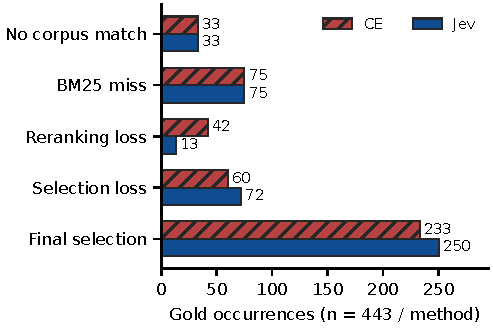
\includegraphics[width=\linewidth]{research/chapter4/figures/section-figures-v1/fig_4_5_gold_loss_stages_column.pdf}
\caption{문항별 gold 출현 443건의 배타적 단계 분류. 미선택은 목록별 선택 수 제약의 영향도 받는다.}
\label{fig:ch4_5}
\end{figure}

개선·CE 우세·지표 불일치 집단에서 F1 차이 절댓값이 각 집단의 중앙값에 가장 가까운 문항을 대표 사례로 선정하였다. 식품 생산실적과 회수계획의 보고 상대방을 묻는 개선 사례에서는 Jev가 식품위생법 제42조제2항을 유지하면서 제45조제1항을 추가로 확보하였다. 근거 F1은 50$\to$100, LF-Eval은 65.29$\to$99.18로 높아졌다. 반면 복수 당사자 청구 절차 사례에서는 정답 근거인 민사소송법 제79조제1항이 Jev의 shortlist에서 탈락하고 제83조제1항이 선택되었다. 답변의 절차 설명도 달라져 F1은 80$\to$40, LF-Eval은 71.79$\to$52.67로 낮아졌다.

사면과 복수 범죄 처리 사례는 gold 3개에 후보 목록이 2개뿐이어서 모든 근거를 선택할 수 없었다. gold 중 하나는 corpus 미매핑, 하나는 BM25 미회수였으며, Jev는 CE가 선택한 나머지 gold도 확보하지 못했다. 근거 F1은 40$\to$0으로 낮아졌지만 Token F1은 18.60$\to$25.88로 상승하였다. 표현 중복의 증가가 더 나은 근거 선택을 보장하지 않음을 보여준다. 이러한 사례는 자동 관측에 근거하며, 정답 외 조문의 법률적 부적절성이나 실제 주장 미지지를 확정한 것은 아니다. 사례 식별자·원문·선정 규칙은 보충자료에 제시하였다.
